\section{ON STATION}

\subsection{Fix Point, Scan responsibilities and splitting}

A CAP station is nothing more than a Hold point with a directional element for
sensors.

\sidebyside{0.625}{
  \textbf{CAPs are to be run at maximum conserve fuel speed.}

  Altitudes generally are high enough to secure fuel conservation whilst
  managing sensor deployment effectively, i.e. look-down shoot-down.

  High altitudes compete with the element of "low surprise". This is the
  balance that is struck. Low CAPs do exist, and the mission will define the
  legs, direction and altitude of the CAP, with 20,000 feet being a reasonable
  compromise.

  Holding Points are based on the specific waypoint being the point of the
  first turn, and several minute legs each way to maintain a steady point above
  ground. Somewhat longer legs than the standard two-minute legs are useful as
  these two minutes can be busy with scans.
}{%
  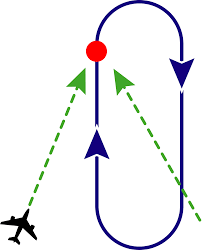
\includegraphics[width=\textwidth,align=t]{aar/cap}%
}

The sensor mate "contract" should already be in effect ever since the FENCE
check incoming, however, to refresh, check that all altitude blocks are covered
with the razors edge crossed by 5,000 feet and the Wingman scanning near and
low blocks, the lead covering far and high. Mating can be also done by Hooking
a Waypoint or item ahead and watching the altitude block.

Whist Normal doctrine requires a flight maintain integrity at all times,
DataLink and Yardstick are technologies that enhance the distance that a flight
could split and splitting the flight to cover hot legs at all times makes a lot
of sense, additionally providing the ability to get into a number of tactical
formations in time for a BVR engagement. For this reason, the length of the
track legs should be the maximum trail length in a split trail engagement, and
no more than mutual support can be inconvenienced, which can be anywhere from 5
to 20nm for Sidewinder, versus Phoenix.
